\subsection{UI und UX Design}
\setauthor{Zoe Emily Öllinger}

Das Design des Frontends wurde zu Beginn in Figma ausgearbeitet und weiters durch absprache und Feedback-Runden verbessert.

\subsubsection{Iteration 1:}
\setauthor{Zoe Emily Öllinger}

Im ersten Meeting mit der Firma wurden uns die Anforderungen für unsere Anwendung dargelegt und es wurde gebeten, zwei verschiedene Workflows zu entwickeln.
Dabei benötigen wir eine Übersichtsseite und eine Detailseite sowie einen Weg um zur Dokumentation in Confluence zu kommen und weiters eventuell auch Statistiken.

\subsubsection{Workflow-Version 1}
\setauthor{Zoe Emily Öllinger}

\begin{figure}[h]
    \centering
    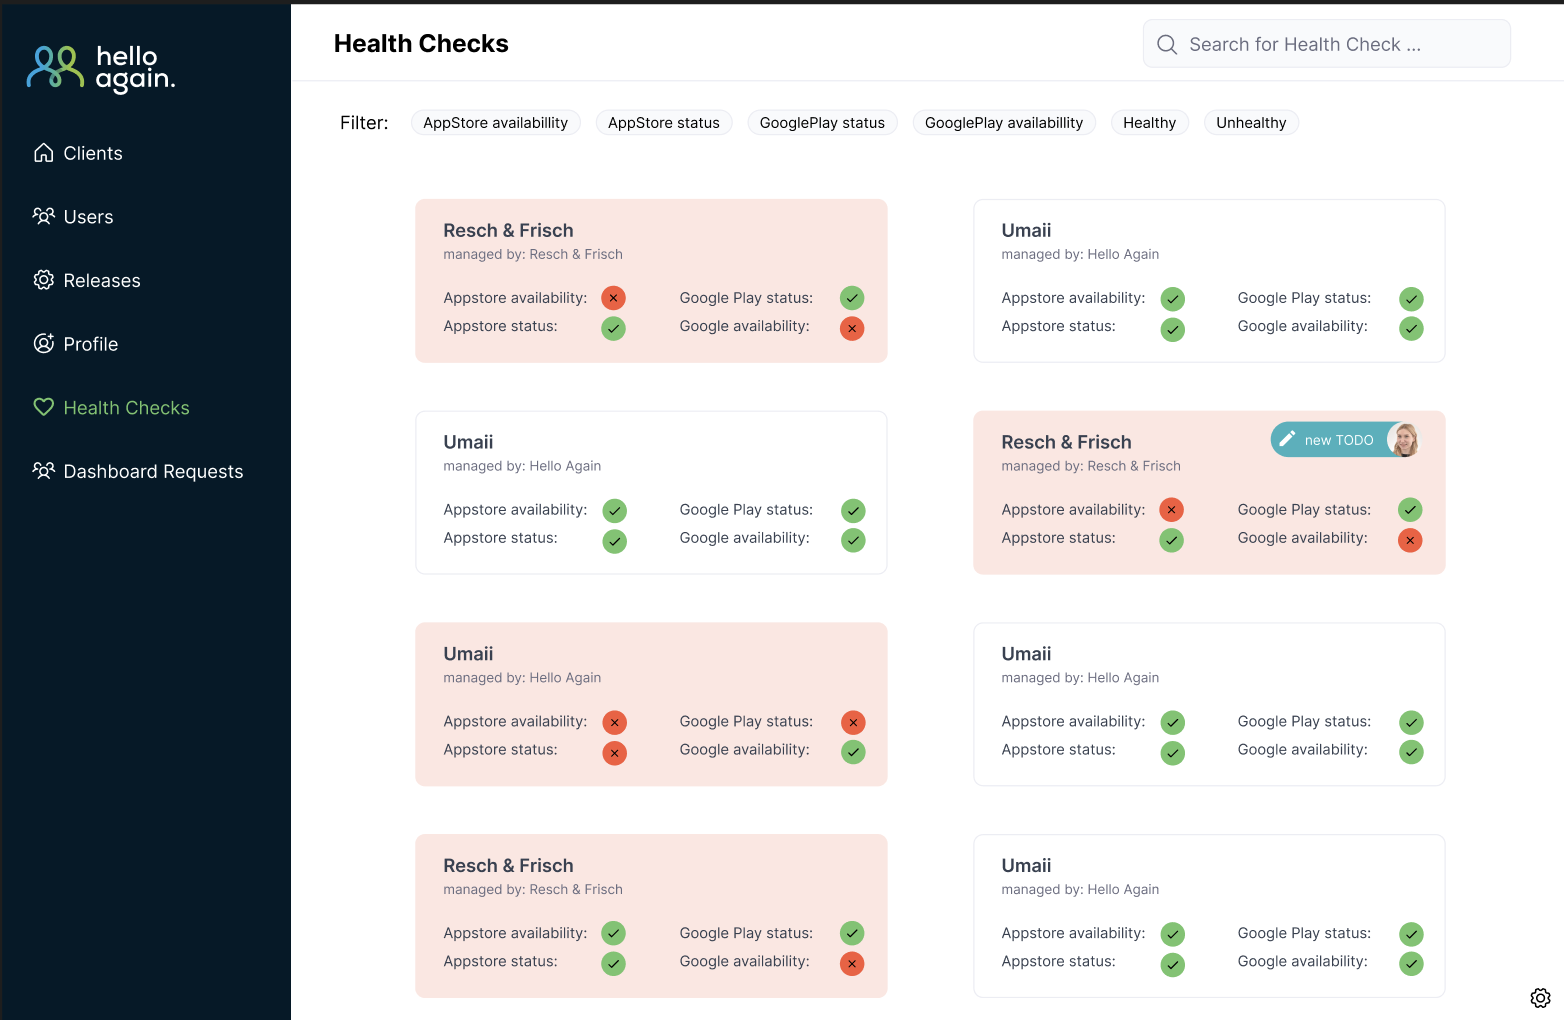
\includegraphics[width=0.8\textwidth]{pics/V1}
    \label{fig:version-1.1-des-dashboards}
\end{figure}

Dies ist die erste Version der Übersichtsseite.
Hier werden die verschiedenen Kunden angezeigt, sowie ein grober Überblick über die Health-Stati.
Je nach Farbe wird angezeigt ob die jeweiligen Apps Healthy oder Unhealthy sind (also ob sie Error werfen oder nicht).
Sobald eine App ausfällt wird sie sofort gekennzeichnet, damit die Mitarbeiter auch dementsprechend auf diese Ausfälle reagieren können.

\begin{figure}[h]
    \centering
    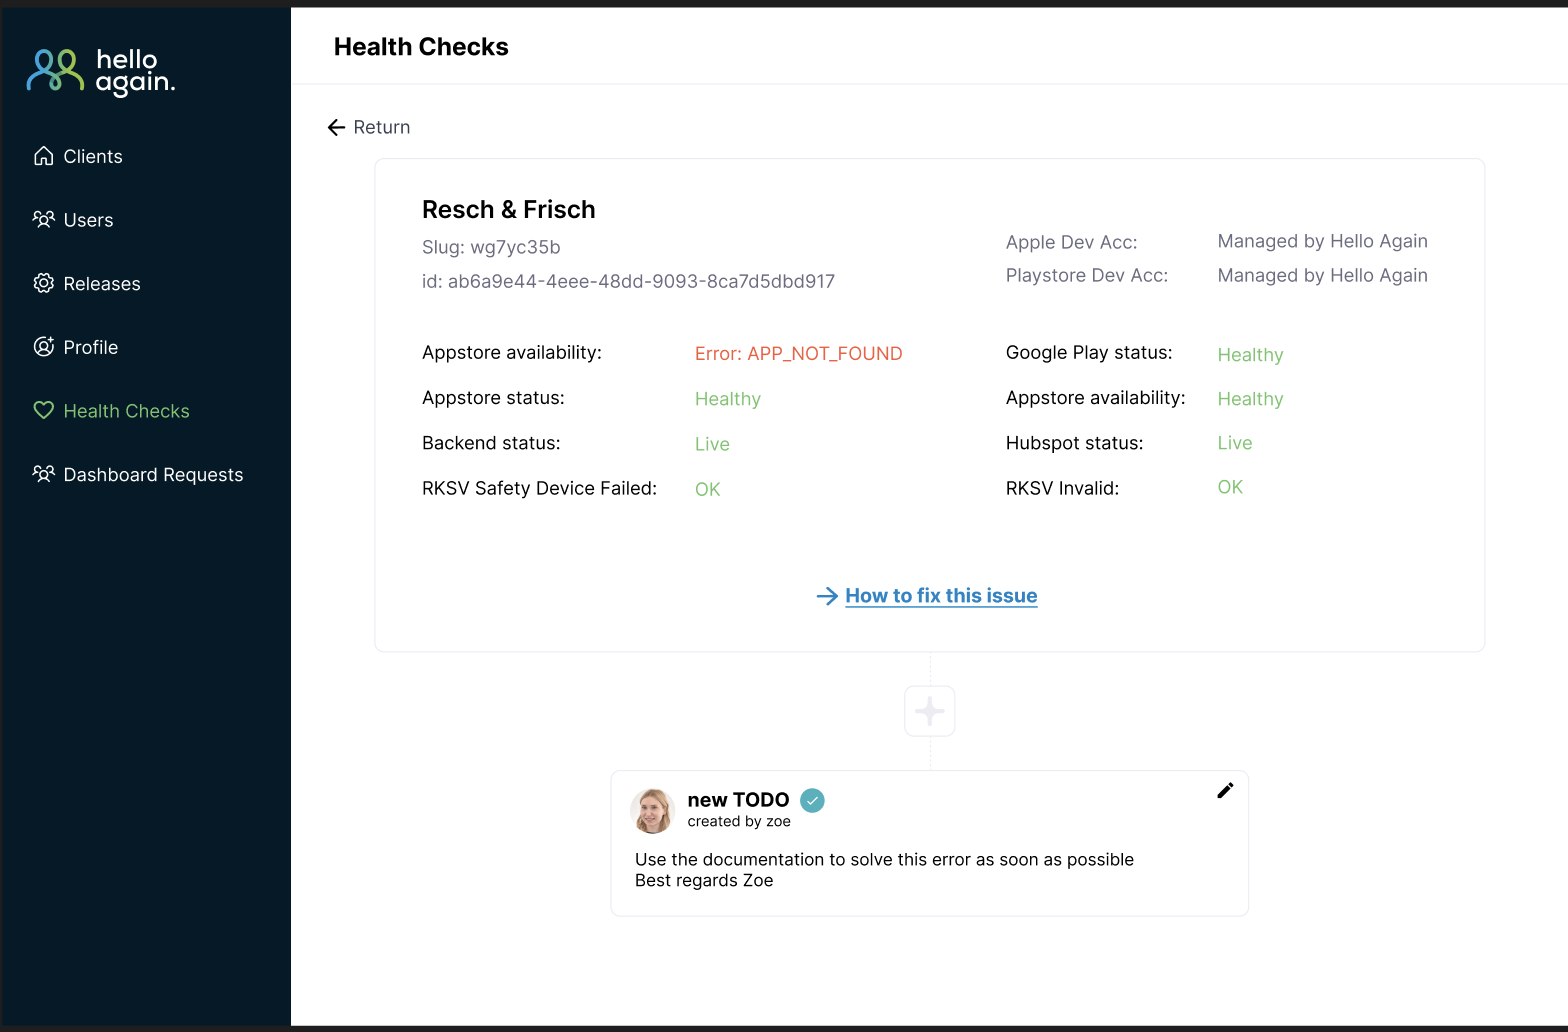
\includegraphics[width=0.8\textwidth]{pics/V2}
    \label{Version 1.2 des Dashboards}
\end{figure}

Dies ist die erste Version der Detailseite, auf der nochmal genauere Daten der Kunden angezeigt werden, sowie den Health-Status der einzelnen Health-Checks. Wird ein Fehler gemeldet wird auf der Detailsseite auch automatisch der Link angezeigt zur Lösung des Errors. Dies ermöglicht den Mitarbeitern eine effiziente und schnelle Arbeitsweise. Weiter unsen sehen wir noch eine TODO-Funktion. Hier kann man direkt im Dashboard Kommentare schreiben, die dann Plattformübergreifend in Asana erstellt werden.

\subsubsection{Workflow-Version 2}
\setauthor{Zoe Emily Öllinger}

\begin{figure}[h]
    \centering
    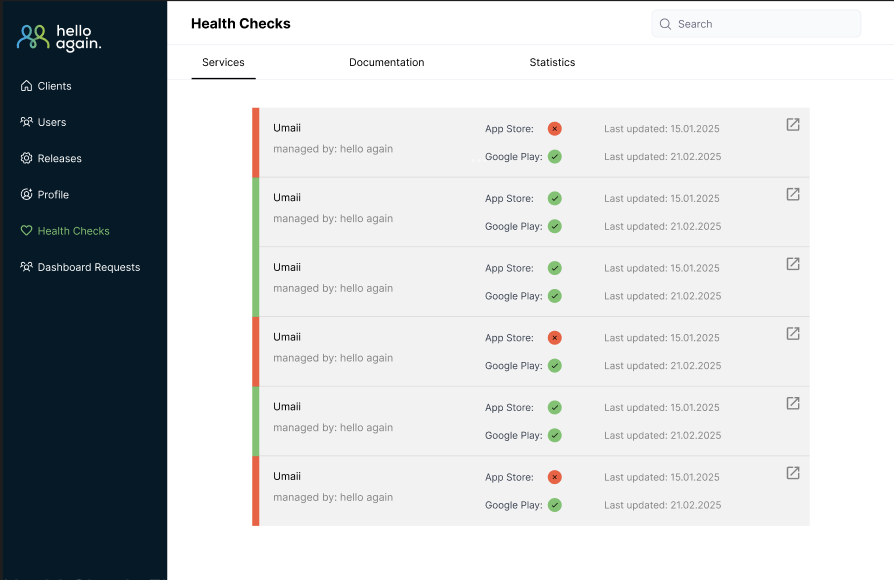
\includegraphics[width=0.8\textwidth]{pics/V3}
    \label{Version 2.1 des Dashboards}
\end{figure}

Dies ist die zweite Workflow-Version die erarbeitet wurde.
Hier haben wir ebenfalls eine Übersichtsseite mit einer Liste doch mit einem kleinen Unterschied.

\begin{figure}[h]
    \centering
    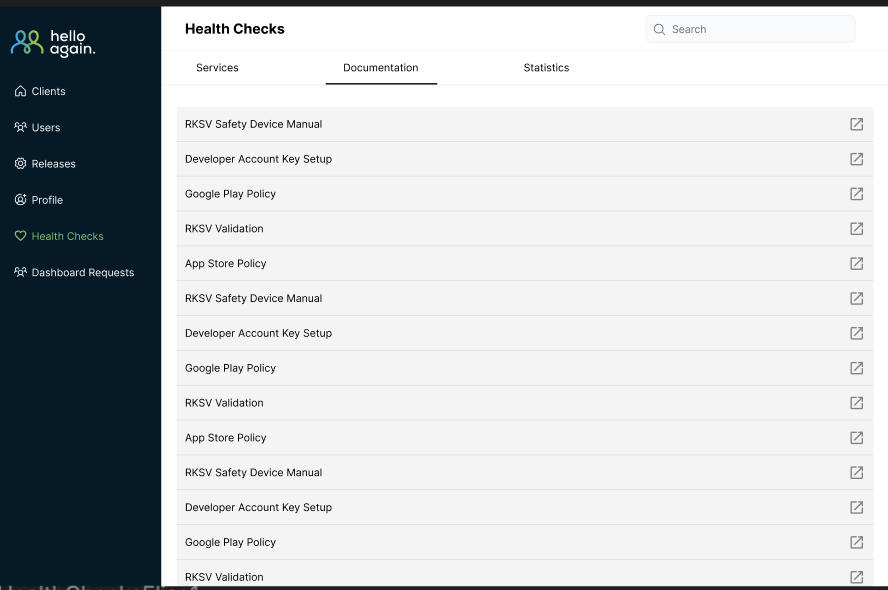
\includegraphics[width=0.8\textwidth]{pics/V4}
    \label{fig:version-2.2-des-dashboards}
\end{figure}

Um zu Dokumentationsseite zu gelangen kann der Tab gewechselt werden, allerdings werden hier alle vorhandenen Dokumentationen zur Fehlerbehebung angezeigt.

\begin{figure}[h]
    \centering
    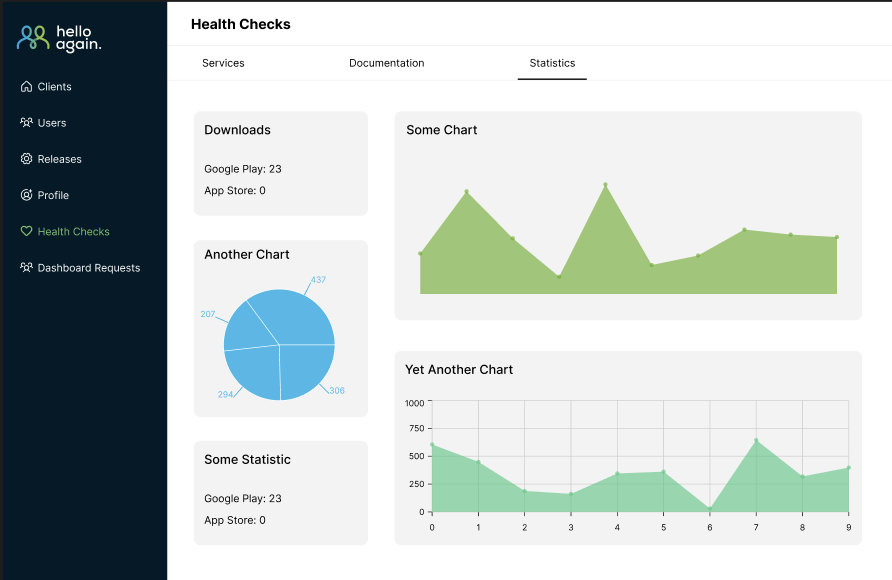
\includegraphics[width=0.8\textwidth]{pics/V5}
    \label{Version 2.3 des Dashboards}
\end{figure}

Als dritten Tab wurde eine Statistik-Übersicht eingebaut bei der man die Downloads der letzten Tage sieht, sowie die Anzahl der App-Ausfälle, damit man potenzielle Fehlerquellen zeitnahe erkennen und beseitigen kann.

\begin{figure}[h]
    \centering
    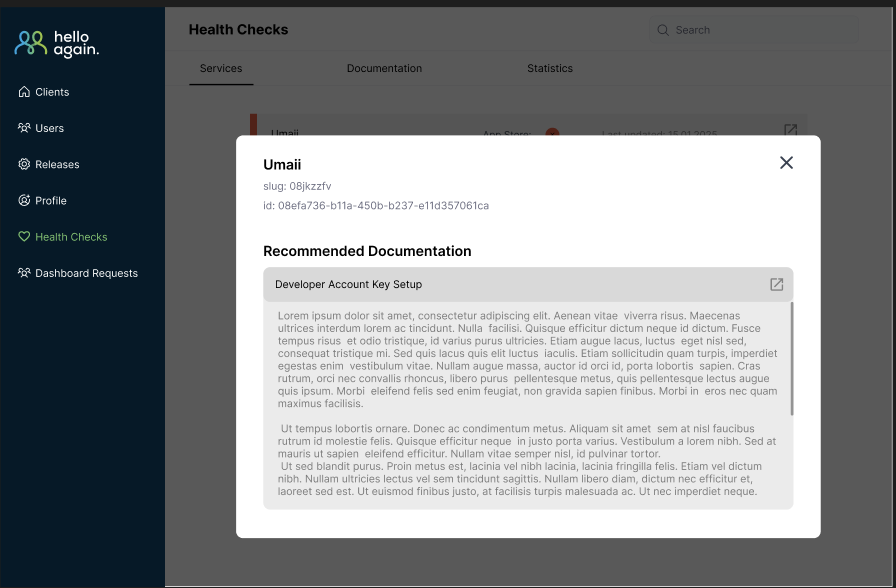
\includegraphics[width=0.8\textwidth]{pics/V7}
    \label{Version 2.4 des Dashboards}
\end{figure}

Die Detailseite sieht sehr ähnlich aus zum ersten Workflow-Konzept allerdings mit dem Unterschied, dass man die Detailseite als Popup sieht.
Unten rechts erscheint ein Button mit dem Namen Resolve Errors.
Klickt man auf diesen, wird ein Fenster angezeigt, dass uns die Dokumentation zur Fehlerbehebung liefert.

\subsubsection{Iteration 2:}
\setauthor{Zoe Emily Öllinger}

Zur Vorstellung beider Konzepte wurden wir in die Firma eingeladen und haben diese dort auch Vorgestellt.
Es wurde schnell klar, dass wir eine Übersichtsseite sowie eine Detailseite brauchen würden mit einer erweiterten Kommentarfunktion und einem Link zur externen Fehlerbehebung, darum wurde sich auf eine Misch-Version der beiden Workflows geeinigt.
Allerdings musste die Liste aller Kunden auf der Übersichtsseite noch etwas schmaler und informativer werden.

\begin{figure}[h]
    \centering
    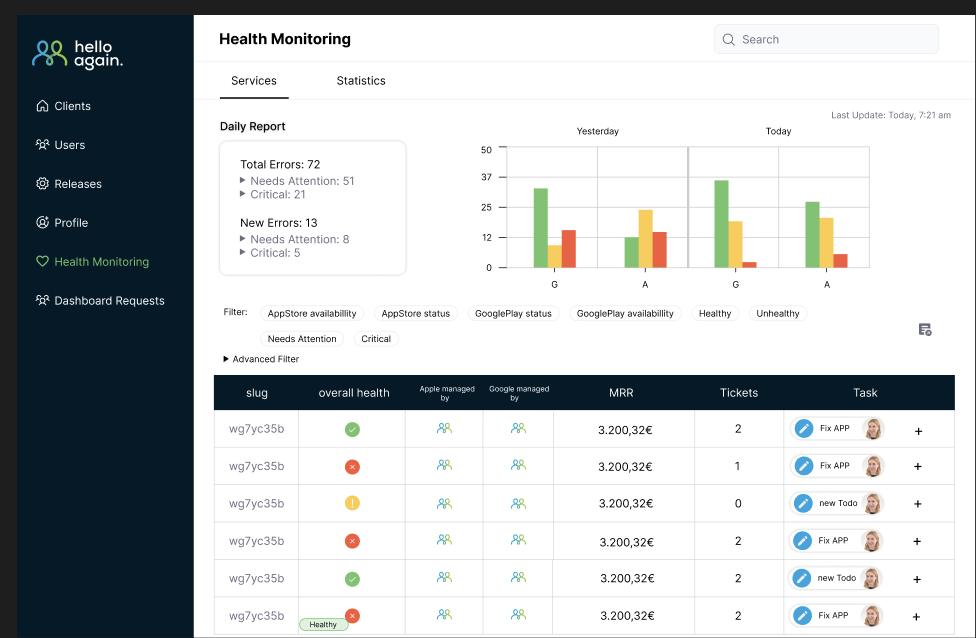
\includegraphics[width=0.8\textwidth]{pics/V9}
    \label{Version 3.1 des Dashboards}
\end{figure}

Hier sehen wir das verbesserte Dashboard-Design, dass nach dem ersten Feedback-Gespräch zustande kam.
Es wurde eine Übersichtliche Statistik eingearbeitet sowie eine schmalere Liste mit mehr nützlichen Informationen für die Mitarbeiter.
Dazu wurden noch Quickfilter eingebaut, die ermöglichen sollen, dass man schnell alle fehlerhaften Apps herausfiltern kann, damit die Zeit, die die App nicht im Appstore verfügbar ist, so klein wie möglich gehalten wird, um so wenig potenziellen Umsatz wie möglich zu verlieren.
Dazu gibt es noch die Advanced-Filter Option.
Diese ist dafür da um nach konkreten Fehlern filtern zu können.
Wenn man zum Beispiel weiß, dass das Liscenseagreement von Google geändert wurde, kann man mit den Advanced-Filtern danach suchen und diese Fehler beheben.
Beim Overall-Health-Status wurde noch eine dritte Option eingführt neben Healthy und Healthy.
Diese heißt Needs-Attention, dass heißt die App könnte bald aus dem Appstore oder Googleplaystore entfernt werden, da Lizenzen abgelaufen sind.
Auch ein Schnellzugriff auf die TODOS soll gewährleistet sein.

\begin{figure}[h]
    \centering
    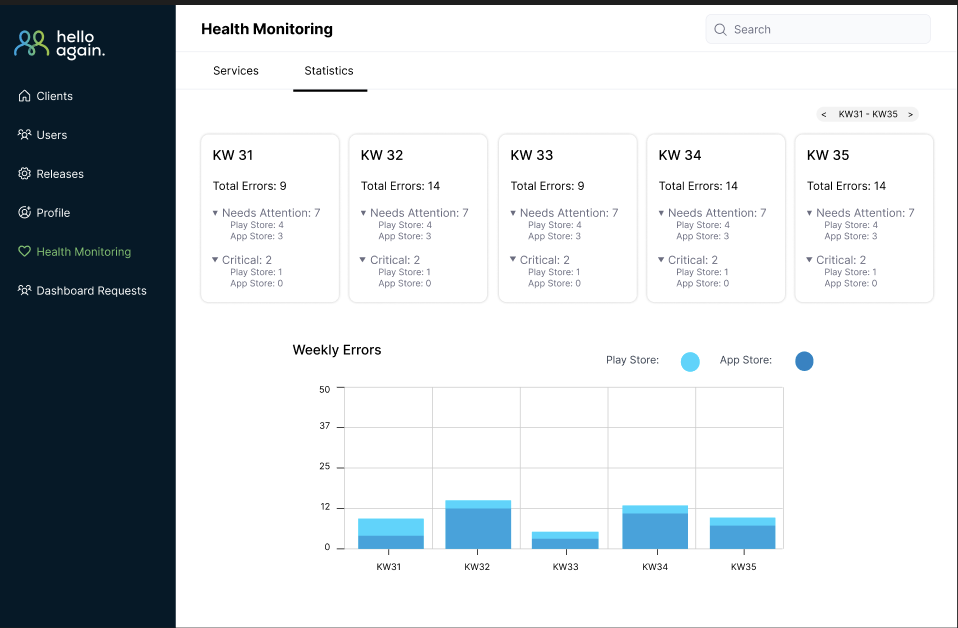
\includegraphics[width=0.8\textwidth]{pics/V8}
    \label{Version 3.2 des Dashboards}
\end{figure}

Weiters gibt es einen eigenen Tab, der die Statistiken auf der Übersichtsseite nochmals erweitert und mit mehr Informationen darstellt.

\begin{figure}[h]
    \centering
    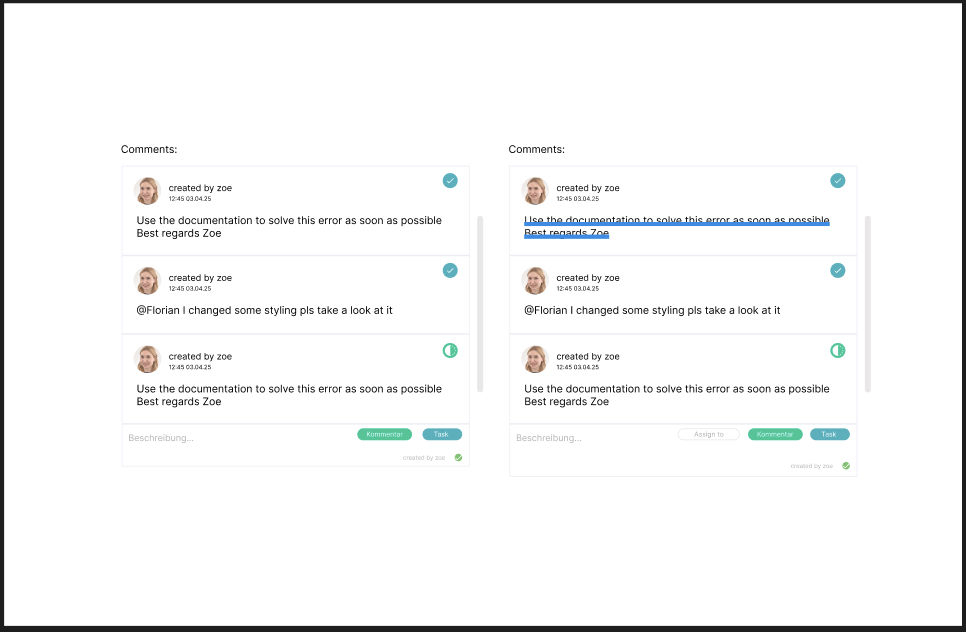
\includegraphics[width=0.8\textwidth]{pics/V12}
    \label{Version 3.3 des Dashboards}
\end{figure}

Dazu wurde die Kommentar- und TODO-Funktion nochmals überarbeitet in zwei verschiednen Version, hier wurde sich schlussendlich für diese Version (siehe Bild oben) entschieden.
